\documentclass[12pt]{article}
\usepackage[utf8]{inputenc}
\usepackage{float}
\usepackage{amsmath}


\usepackage[hmargin=3cm,vmargin=6.0cm]{geometry}
%\topmargin=0cm
\topmargin=-2cm
\addtolength{\textheight}{6.5cm}
\addtolength{\textwidth}{2.0cm}
%\setlength{\leftmargin}{-5cm}
\setlength{\oddsidemargin}{0.0cm}
\setlength{\evensidemargin}{0.0cm}

%misc libraries goes here
\usepackage{tikz}


\begin{document}

\section*{Student Information } 
%Write your full name and id number between the colon and newline
%Put one empty space character after colon and before newline
Full Name :  Burak Bahar\\
Id Number :  2380137\\

% Write your answers below the section tags
\section*{Answer 1}
a)
\begin{figure}[H]
	\centering
	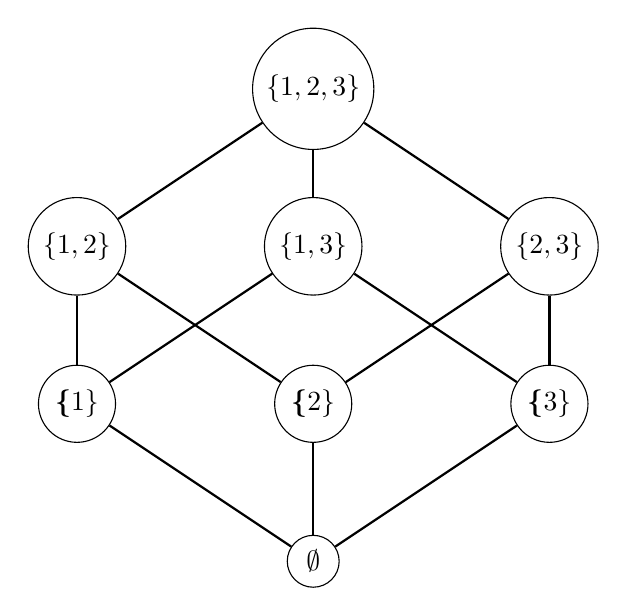
\begin{tikzpicture}
	
	\node[shape=circle,draw=black] (a) at (3, 0)     {\textbf{$\emptyset$}};
	\node[shape=circle,draw=black] (b) at (0, 2)     {\textbf\{1\}};
	\node[shape=circle,draw=black] (c) at (3, 2)     {\textbf\{2\}};
	\node[shape=circle,draw=black] (d) at (6, 2)     {\textbf\{3\}};
	\node[shape=circle,draw=black] (e) at (0, 4)     {\textbf{$\{1,2\}$}};
	\node[shape=circle,draw=black] (f) at (3, 4)     {\textbf{$\{1,3\}$}};
	\node[shape=circle,draw=black] (g) at (6, 4)     {\textbf{$\{2,3\}$}};
	\node[shape=circle,draw=black] (h) at (3, 6)     {\textbf{$\{1,2,3\}$}};
	
	\path[-, thick] (a) edge (b);
	\path[-, thick] (a) edge (c);
	\path[-, thick] (a) edge (d);
	\path[-, thick] (b) edge (e);
	\path[-, thick] (c) edge (e);
	\path[-, thick] (b) edge (f);
	\path[-, thick] (d) edge (f);
	\path[-, thick] (c) edge (g);
	\path[-, thick] (d) edge (g);
	\path[-, thick] (e) edge (h);
	\path[-, thick] (f) edge (h);
	\path[-, thick] (g) edge (h);
	\end{tikzpicture}
\end{figure}
b) Yes it is. It has least upper bound, greatest lower bound.\\
c) \{1,2,3\} \\
d) $\emptyset$ \\
e)Yes. \{1,2,3\}  \\
f)Yes. $\emptyset$ \\
g) \{1,3\}

\section*{Answer 2}
a) deg(a) = 2 \\ deg(b) = 4 \\ deg(c) = 2\\  deg(d) = 3 \\ deg(e) = 3 \\ sum = 14 \\
b)For every vertex the edge between them will be counted 2 times.Edge num = 7. So, 7*2=14.\\
c) For every edge there will 2 two 1 in the incident matrix's columns.So, again 7*2 =14 \\
d) yes there is.
\begin{figure}[H]
	\centering
	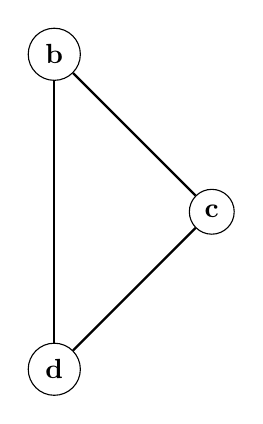
\begin{tikzpicture}
	
	
	\node[shape=circle,draw=black] (b) at (4, 4)     {\textbf{b}};
	\node[shape=circle,draw=black] (c) at (6, 2)     {\textbf{c}};
	\node[shape=circle,draw=black] (d) at (4, 0)     {\textbf{d}};
	
	\path[-, thick] (b) edge (c);
	\path[-, thick] (b) edge (d);
	\path[-, thick] (d) edge (c);
	
	\end{tikzpicture} 
\end{figure}
e) No it is not. b has an edge to every other vertices, but the other vertex is still connected to each other.if (b,d) and (a,e) is gone.It will be bipartite with one side (b,d) the other (a,e,c). \newline
f) Every edge can be in, out or both. Additionally we are choosing this for every edge. There are 7 edges. So, $7^3$. \newline
g) It is 4. Going every vertex once is 4 edge. For example, a,b,c,d,e.\newline
h) 1 since it is connected graph.\newline
i) Since from theorem, not all vertices have even degree, it doesn't have Euler circuit.\newline
j) e,b,d,c,b,a,e,d\newline
k) b,a,e,d,c,b\newline
l) b,a,e,d,c\newline


\section*{Answer 3}
\paragraph{I noticed that in G every vertex in the outside square is connected to to inner vertex, and just two edge goes to a inner vertex. I determined these inner edges' connections and placed them like in H, by placing them between the vertices that connects them in outer square. So, yes, they are isomorphic.}

\section*{Answer 4}
\paragraph{In this solution the columns are the step that lock the vertices. Each column will lock one vertex and a, as initial point will start as locked. The locked vertices and not initialed vertices will be represented with "-" in the columns. The most left column indicate the order I lock the vertices.\\
For each step I write the possible accessible vertices and the shortest way to them. I lock the smallest number in each step until all is locked. Answer = a,b,c,f,j  }
\paragraph{$1 |$ $a |$ $0 |$ $ - |$ $- |$ $ - |$ $ - |$ $ - |$ $ - |$ $ - |$ $ - |$ $ - |$ $ - |$ 0 \\
$2 |$ $  b |$ $ 3 |$ $ - |$ $ - |$ $ - |$ $ - |$ $ - |$ $ - |$ $ - |$ $ - |$ $ - |$ $ - |$ 3 \\
$4 |$ $  c |$ $ - |$ $ 5 | $ $ 5 | $ $ - |$ $ - |$ $ - |$ $ - |$ $ - |$ $ - |$ $ - |$ $- |$5 \\
$8 |$ $  d |$ $ - |$ $ - |$ $ - |$ $ 8 |$ $ 8 |$ $ 8 |$ $ 8 |$ $ - |$ $ - |$ $ - |$ $ - |$ 8 \\
$5 |$ $  e |$ $ 5 |$ $ 5 |$ $ 5 |$ $ 5 |$ $ - |$ $ - |$ $ - |$ $ - |$ $ - |$ $ - |$ $ - |$ 5 \\
$7 |$ $  f |$ $ - |$ $ 10|$ $ 9 |$ $ 7 |$ $ 7 |$ $ 7 |$ $ - |$ $ - |$ $ - |$ $ - |$ $ - |$ 7 \\ 
$11|$ $  g |$ $ - |$ $ - |$ $ - |$ $ 11|$ $ 11|$ $ 11|$ $ 11|$ $ 11|$ $ 11|$ $ 11|$ $ - |$ 11 \\
$9 |$ $  k |$ $ - |$ $ - |$ $ - |$ $ - |$ $ - |$ $ - |$ $ - |$ $ 10|$ $ - |$ $ - |$ $ - |$ 10\\
$3 |$ $  h |$ $ 4 |$ $ 4 |$ $ - |$ $ - |$ $ - |$ $ - |$ $ - |$ $ - |$ $ - |$ $ - |$ $ - |$ 4 \\
$6 |$ $  i |$ $ - |$ $ - |$ $ 6 |$ $ 6 |$ $ 6 |$ $ - |$ $ - |$ $ - |$ $ - |$ $ - |$ $ - |$ 6 \\
$10|$ $  j |$ $ - |$ $ - |$ $ - |$ $ - |$ $ - |$ $ 10|$ $ 10|$ $ 10|$ $ 10|$ $ - |$ $ - |$ 10\\}

        
\section*{Answer 5}
\paragraph{I used Prim's algorithm.\\
a)a,b,d,c,f,e\\}
b)a as root. \begin{figure}[H]
	\centering
	\begin{tikzpicture}
	
	\node[shape=circle,draw=black] (a) at (3, 6)     {\textbf{a}};
	\node[shape=circle,draw=black] (b) at (5, 4)     {\textbf{b}};
	\node[shape=circle,draw=black] (c) at (7, 2)     {\textbf{c}};
	\node[shape=circle,draw=black] (d) at (1, 4)     {\textbf{d}};
	\node[shape=circle,draw=black] (e) at (4, 2)     {\textbf{e}};
	\node[shape=circle,draw=black] (f) at (6, 0)     {\textbf{f}};
	
	\path[-, thick] (a) edge node[above]{1} (b);
	\path[-, thick] (b) edge node[above]{4} (c);
	\path[-, thick] (a) edge node[right]{3} (d);
	\path[-, thick] (b) edge node[right]{5} (e);
	\path[-, thick] (c) edge node[left]{2} (f);
    \end{tikzpicture} 
\end{figure}
\paragraph{c) No we can simple change the root. For example if we choose b as root tree will just hang from b instead of a. Additionally if we choose f as root there will be a different tree but still the sum of weight will be the same as the tree in b.}

\section*{Answer 6}
\paragraph{\\
a) 13 vertices, 12 edge and height is 4 \\
b) w,s,m,t,q,x,n,y,u,z,v,r,p \\
c) s,w,q,m,t,p,x,u,n,y,r,v,z \\
d) p,q,s,w,t,m,r,u,x,y,n,v,z \\
e) No, not every node has 2 children.}


\end{document}